\clearpage
\section{Základy šifrování}
\subsection{Vysvětlete pojmy kryptografie, kryptoanalýza a kryptologie. Jaké hlavní úkoly plní kryptografické systémy? Jaké základní typy operací používá?}
\begin{itemize}
    \item \textbf{Kryptografie} - Věda zabývající se problematikou navrhování šifrovacích metod.
    \item \textbf{Kryptoanalýza} - Věda zabývající se luštěním zašifrovaných textů bez znalosti tajného klíče (prolamování)
    \item \textbf{Kryptologie} - Věda zabývající se studiem problematiky šifrování a dešifrování
    \item \textbf{Důvěrnost} - Utajení informace před neoprávněnými uživatelem. \textbf{Autentičnost} - Příjemce má možnost zjistit původ zprávy. \textbf{Integrita} - Kontrola zprávy, zda nebyla během přenosu modifikována. \textbf{Nepopiratelnost} - Odesílatel by neměl mít možnost popřít autorství zprávy.
    \item Jednoduché aritmetické operace (operace součtu modulo dvě), Substituce (znak původní zprávy se nahradí definovaným způsobem jiným znakem), Permutace (změní se definovaným způsobem pořadí znaků ve zprávě)
\end{itemize}

\subsection{Zakreslete a popište schéma kryptografického systému.}
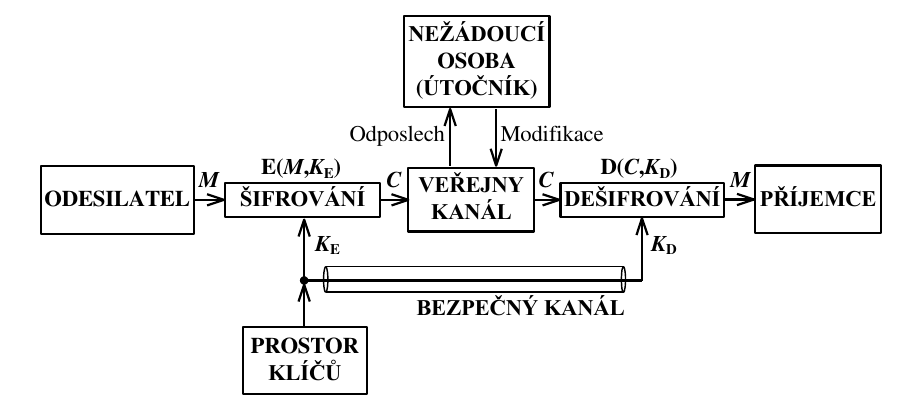
\includegraphics[width=16cm]{images/12_schema.png}

\subsection{Jaké jsou základní pravidla kryptografie?}
\begin{itemize}
    \item Šifrovací systém má být navržen tak, aby bylo snadné měnit šifrovací klíč nebo šifrovací postup.
    \item Nepovolaná osoba smí mít k dispozici minimální množství šifrovaných dat. Data, která nejsou tajná,
    se zabezpečovat šifrou nemají.
    \item  V žádném případě nesmí dojít k tomu, že by se tatáž zpráva přenášela vícekrát, při čemž by byla 
    pokaždé zašifrována stejným klíčem.
    \item Užívá-li se ke generování šifrovacího klíče nějaká pseudonáhodná posloupnost čísel, je
    třeba tato čísla generovat postupem, o kterém víme, že jej nežádoucí osoba nezná.
\end{itemize}

\subsection{Uveďte základní typy operací využívaných v kryptografii?}
\begin{itemize}
    \item \textbf{Aritmetické operace} - data jsou brána jako čísla
    \item \textbf{Substituce} - data se nahrazují jinými
    \item \textbf{Transpozice} (Permutace) - Mění pořadí znaků ve zprávě
\end{itemize}

\subsection{Symetrické a asymetrické kryptosystémy (varianty), výhody + příklad použití}
\textbf{Symetrické}
\begin{itemize}
    \item Systémy s tajným, jediným klíčem
    \item Používají se v případech dvoubodového spoje
    \item\textbf{  - }Problém distribuce klíče (DH), Nelze prokázat totožnost autora zašifrovaných dat
    \item\textbf{ + }Velmi rychlé algoritmy, šifrování velkých objemů dat.
    \item Caeserova šifra, Vigenérova šifra (substituce), DES, AES
\end{itemize}
\textbf{Asymetrické}
\begin{itemize}
    \item Systémy s veřejným klíčem, klíče jsou navzájem různé a výpočet Kv → Ks je prakticky nerealizovatelný
    \item Jeden klíč je veřejný (zajištění důvěrnosti a integrity)  a druhý tajný (zajištění autentičnost dat)
    \item Využití problému faktorizace velkých čísel, diskrétního logaritmu, eliptických křivek
    \item  K podepisování zpráv a k distribuci klíčů pro symetrické kryptosystémy
    \item\textbf{ - }Pomalejší, zapotřebí infrastruktura veřejných klíčů 
    \item\textbf{ + }Umožňuje zajištění důvěrnosti, integrity a autentičnosti dat 
    \item RSA, DH
\end{itemize}

\subsection{Stručně popište kryptosystémy DES a AES.}

\subsection{Stručně popište metodu RSA. Na čem je založena její bezpečnost?}

\subsection{Stručně popište metodu Diffie-Hellman a uveďte příklady využití.}

\subsection{Co je to digitální otisk (heš). Vysvětlete využití.}